% !TeX program = lualatex
% !TeX encoding = UTF-8
% !TeX spellcheck = fr_FR
% !TeX root = main.tex
% Source : https://fr.overleaf.com/latex/templates/template-defesa-ipb-utfpr/dcyxxfxxwfmv

\documentclass[xcolor={dvipsnames}]{beamer}

\usepackage[colorinlistoftodos,french]{todonotes}
\usepackage[french]{babel}
\usepackage{multimedia}

\setcounter{tocdepth}{1}

% Mettre les todos en lignes plutôt qu'en marge de la page
\presetkeys{todonotes}{inline}{}

\setbeamerfont{author}{size=\Large}

\mode<presentation> {

    \usetheme{Madrid}
    \usecolortheme[named=Farbe]{} % use a pre defined theme
    %\usecolortheme{ipbutfpr} % use a custom color theme
    % http://mcclinews.free.fr/latex/introbeamer/elements_diaporama.html

    \setbeamertemplate{caption}[numbered]
    \setbeamertemplate{frametitle continuation}{\gdef\beamer@frametitle{}}

    \setbeamertemplate{footline}{
        \leavevmode%
        \hbox{%
            %\begin{beamercolorbox}[wd=.4\paperwidth,ht=2.25ex,dp=1ex,center]{author in head/foot}%
            %    \usebeamerfont{author in head/foot}\insertshortauthor
            %\end{beamercolorbox}%
            \begin{beamercolorbox}[wd=1\paperwidth,ht=2.25ex,dp=1ex,center]{title in head/foot}%
                \usebeamerfont{title in head/foot}\insertshorttitle\hspace*{6em}
                \insertframenumber{} / \inserttotalframenumber\hspace*{1ex}
            \end{beamercolorbox}
        }%
        \vskip0pt%
    }

    \setbeamertemplate{navigation symbols}{}
    \usepackage{pgfpages}
    \setbeameroption{show notes on second screen=right}
	%\setbeameroption{show only notes}
    %\setbeameroption{hide notes}

	\definecolor{inversevideodessous}{rgb}{0.0, 0.28, 0.67}
	\definecolor{inversevideodessus}{rgb}{1,1,1}
	\usesectionheadtemplate
	{\colorbox{inversevideodessous}{\color{inversevideodessus} \insertsectionhead}}
	{\color{inversevideodessous} \insertsectionhead}
	
	\defbeamertemplate*{headline}{}
	{%
		\begin{beamercolorbox}[ht=1.875ex,dp=0.75ex]{section in head/foot}%
			\insertsectionnavigationhorizontal{\paperwidth}{}{}%
		\end{beamercolorbox}%
		\begin{beamercolorbox}[ht=1.875ex,dp=0.75ex]{subsection in head/foot}
			\usebeamerfont{subsection in head/foot}
			\insertsubsectionnavigationhorizontal{\paperwidth}{}{\hskip0pt plus1filll}%
		\end{beamercolorbox}%
	}    
}

\title[Automatisation \& amélioration du cycle de vie d'une application]{Comment l’automatisation peut-elle permettre d’améliorer le cycle de vie d’une application ?}
\author{Sylvain METAYER}

\institute{\normalsize
    \begin{figure}[htb]
        \centering
        
\includegraphics[width=0.35\textwidth]{img/onepoint.jpg}
        
\includegraphics[width=0.35\textwidth]{img/epsi.jpg}
    \end{figure}
}

\date{\small 4 Septembre 2019 \\ 11h}

\begin{document}
    \frame[plain]{\titlepage}
    
    \begin{frame}[plain]{Plan}
    	\tableofcontents
	\end{frame}      

	%-----SLIDES-----%
	\todo{Introduction, 5-6 pages}

\todo{Quand la partie introduction sera terminée, supprimer les parties.}

\subsection{Accroche}
L'automatisation a toujours été perçue comme un moyen de gagner en productivité, temps, et donc de rendre des projets toujours plus rentable.
	
Les projets informatiques sont de plus en plus nombreux, que cela soit des logiciels de bureau, des applications web, ou encore avec les nouveaux terminaux, des applications mobile, tablettes ou même pour montres connectées.
	
Les projets augmentent donc en quantité, mais augmentent-ils en qualité ? Leur fiabilité n'est en effet pas toujours optimale. 
	
Combien de projet sont encore déployé manuellement car aucune automatisation n'est présente sur le projet ? 
	
En plus d'une perte de temps, parfois importante, cela engendre un stress au niveau des équipes de développeurs, qui à chaque livraison redoute les régressions qui pourraient survenir ou encore les bugs de déploiement.

L'automatisation peut également permettre d'améliorer l'arrivée d'un nouveau développeur sur un projet. Il n'est en effet par rare de voir des projets ou la configuration de l'environnement requiert à elle seule plusieurs jours, sans que le développeur puisse vraiment commencer à travailler.
	
L'automatisation va permettre d'améliorer la fiabilité ainsi que la confiance des développeurs et clients dans le projet, puisque des tests automatisés ainsi qu'une chaine d'industrialisation complètement automatisée permet ainsi de déployer avec confiance une application.
	
Nous allons donc tenter de répondre à la problématique suivante :
	
{\LARGE \problematique}

\subsection{Définition}

Avant de continuer, il convient de s'attarder sur ce qu'est l'automatisation.

Selon le Larousse, l'automatisation est le 

\begin{quote}
fait d'automatiser l'exécution d'une tâche, d'une suite d'opérations...
\end{quote}

\subsection{Historique}

Idées : 
	
- Mode opératoire suivi religieusement, 

- script expect

- Comment déployait-on avant ?

-  ...


\textit{L’introduction doit remplir une fonction traditionnelle : délimiter et présenter le projet ou la mission et son contexte professionnel, annoncer les parties principales du développement. L’introduction représente environ un dixième du mémoire. Il faut absolument insister sur la bonne impression qu’elle doit donner au lecteur comme premier et décisif contact avec le mémoire.}

\subsection{Que peut-on automatiser ?}

\subsection{Pourquoi automatiser ?}

Quels en sont les avantages ?

- éviter erreurs développeur

- éviter script executé avec mauvais parmaètres

\subsection{Présentation entreprise / mission}

L'entreprise dans laquelle j'effectue mon alternance depuis septembre 2017 est \onepoint. 

\xmakefirstuc{\onepoint{}} est une \gls{esn} à taille humaine. Son domaine d'activité est d'accompagner ses clients dans leur transformation numérique, 

C'est une \gls{SAS} disposant de 14 implantations dans le monde. L'entreprise a effectué en 2018 un chiffre d'affaire de 300 million d'euros.

Elle dispose de 2300 collaborateurs, en moyenne agé de 33 ans.

\xmakefirstuc{\onepoint{}} se compose de plusieurs communautés.

\begin{itemize}
	\item Des communautés \emph{régions}, permettant de regrouper les collaborateurs par leur proximité géographique.
	\item Des communautés \emph{expertise}, regroupant l'expertise de chacun, et permettant à tous de progresser. On y retrouve par exemple la communauté Sécurité ou encore Architecture.
	\item Des communautés \emph{support}, tel que la \gls{DSI}, ou les Ressources Humaines, nécessaire au fonctionnement de l'entreprise.
	\item Des communautés \emph{métiers}, regroupant des personnes maitrisant les aspects métiers des différents clients, ainsi que les contraintes de ces métiers. Cela peut par exemple être les métiers des Assurances, des Banques, des Télécoms... 
\end{itemize}

Ainsi, lors du développement d'un projet, toutes ces communautés sont utilisés, afin de tirer le meilleur d'entre elle et de regrouper les personnes les plus aptes à réaliser le projet.

Cela implique aussi que chaque collaborateur peut ainsi appartenir à une ou plusieurs communautés, selon ses compétences, expérience et localisation.

\subsubsection{Historique} 

\xmakefirstuc{\onepoint{}} a été créé en 2002, par David Layani.

De 2003 jusqu'en 2007, elle va s'ouvrir à l'international, avec l'ouverture de bureaux au Canada, en Chine et en Tunisie.

En 2008, elle étend sa position en France, avec l'ouverture de deux centres de production, à Bordeaux et Nantes.

En 2015, \onepoint{} continue son développement international au Luxembourg, en Belgique et en Hollande, avant de racheter VisionIT Group.

En 2018, \onepoint{} ouvre des bureaux à Lyon et en Australie, et rachète également Weave ainsi que Géronimo, acteur important dans la conception d'application mobile.

\subsubsection{Réalisations}

\subsubsection{Contexte de l'alternance}

Projet Nouvelle Aquitaine, chaine d'industrialisation pour pouvoir permettre déploiement de multiple sites Drupal.

\textit{Projet \bv{}, ou il y a une architecture actuelle qui n'est pas satisfaisante pour X raisons (reproductibilité...), et qui doit être changé}.

\textit{Elaborer un schéma directeur à partir d’orientations stratégiques} => Conduite de changement


\subsection{Annonce du plan}
	\section[Cycle de vie]{Cycle de vie d'une application}
\subsection{Définition}
\begin{frame}{\subsecname}
	\begin{block}{}
		Ensemble d'étapes intervenant au cours du développement d'un projet informatique
	\end{block}
	\todo{définition rapido à partir du mémoire pour rafraîchir les mémoires}
\end{frame}

\subsection{Cas de la Nouvelle-Aquitaine}

\begin{frame}{Le projet}
	\begin{block}{Des portails web}
		\note{Pour décrire les différents services et aides offerte par la région. Chacun s'adresse à un public différent}
		\begin{itemize}
			\item Transport
			\item Guide des aides
			\item Portail Jeunes
			\item Régie d'Information
			\item Entreprise
			\item ...
		\end{itemize}
	\end{block}
\end{frame}

\begin{frame}{État actuel}
	\todo{Schéma indiquant les différents états des portails. Par exemple, transport a déjà fait un tour complet, ainsi que GDA, certains portails ne sont encore qu'en phase d'étude... }
	\todo{Frames manquantes pour détailler le cycle de vie}
\end{frame}
	\section[Automatisation]{Automatisation du cycle de vie d'une application}

\subsection{Définition}
\begin{frame}{\subsecname}
	\todo{Définition depuis l'intro du mémoire + partie 2.}
\end{frame}

\subsection{Raisons}
\begin{frame}{\subsecname}
	\todo{plusieurs sites à déployer sur NAQ. Soucis de factorisation/ possibilité de pouvoir mettre à disposition du client une version rapidement. Avant : déploiement fait par une ou deux personnes manuellement. Maintenant : déploiement à la demande auto via clic bouton}
\end{frame}

\subsection{Gestion de projet}
\begin{frame}{Partie Financière}
	\begin{columns}[onlytextwidth]
		\column{.47\textwidth}
		\begin{block}{KPI}
			\begin{itemize}
				\item Temps de déploiement réduit
				\item Time to market réduit
				\item PRA
				\item Livrer de la valeur métier plus rapidement
			\end{itemize}
			\note{Exemple sur les projets NAQ, avant déploiements manuels de ~20min/site. Maintenant ~5min par site. Permet de livrer plus rapidment au client, et permet une reprise plus rapide}
		\end{block}
		\column{.47\textwidth}
		\pause
		\begin{figure}
			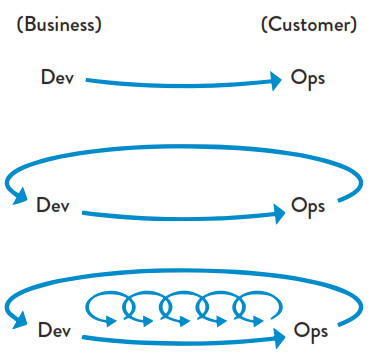
\includegraphics[width=0.9\linewidth]{../img/devops-objective.jpg}
			\caption{Mouvement DevOps}
			\label{fig:devops}
		\end{figure}
	\end{columns}
\end{frame}

\begin{frame}{Organisation}
	\begin{block}{Flux de travail}
		\begin{itemize}
			\item Réduire WIP
			\item Jira
			\item Code review
		\end{itemize}
		\note{Exemple sur les projets NAQ, avant demande qui pouvait trainer plusieurs semaines en attente. Maintenant, on a des demandes qui ne sont pas travaillées tant qu'elles ne sont pas clairemeent définies par le client.}
		\note{Code review qui se met petit à petit en place}
	\end{block}

	\missingfigure{Code review + JIRA}
\end{frame}

\subsection[Développement]{Environnement de développement local}
\begin{frame}{\subsecname}
	IDE
	
	Initialisation ud projet : avant c'était chiant à faire. Maintenant c'est 5 commandes et 10min à peine
\end{frame}

\subsection{Tests}
\begin{frame}{\subsecname}
	Mise en place de POC de test (test unitaire avec mock de composant) \\
	CI test dump de prod pour vérifier que les updates passent bien.
\end{frame}

\section{Mise en place CI/CD}
\begin{frame}{Architecture projet}
	Starterkit pour template de site
	 \\
	 module communs
	 \\
	 thème communs
	 \\
	 un site 
	 \\ gros projet de migration de l'existant qui était fait à la bonne franquette
\end{frame}

\begin{frame}{Architecture projet}
	Starterkit pour template de site
	\\
	module communs
	\\
	thème communs
	\\
	un site 
	\\ gros projet de migration de l'existant qui était fait à la bonne franquette
\end{frame}

\begin{frame}{Gestion de versions}
	Primordial pour différencier les différentes version \\
	avant : manuel \\
	maintenant : auto sur 4 digits. Les deux premiers peuvent être incrémentés auto
\end{frame}

\begin{frame}{Jenkins}
	\missingfigure{Image des jobs jenkins}
	Organisation par portail \\ 
	Job sur SCM \\
	
\end{frame}
	\section{Mise en place CI}
\subsection[Architecture]{Architecture projet}
\begin{frame}{\subsecname}
	\begin{overprint}
		\onslide<1> 
		\begin{block}{Avant}
			\note[item]{Chaque portail différent. Maintenance difficile, impossible de réutiliser des modules d'un site dans un autres.}
			\centering 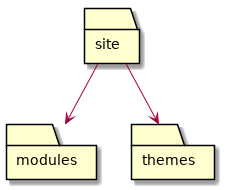
\includegraphics[width=0.25\textwidth]{img/before-drupal.png}
		\end{block}
		\onslide<2> 
		\begin{block}{Après}
			\note[item]{Mise en place d'un modèle de référence pour tous les portails. Regroupement modules communs dans un dépôt à part qui sera exposé sur un artifactory pour être réutilisé par les autres sites, en gérant les versions. Travail de migration de tous les portails existants}
			\centering 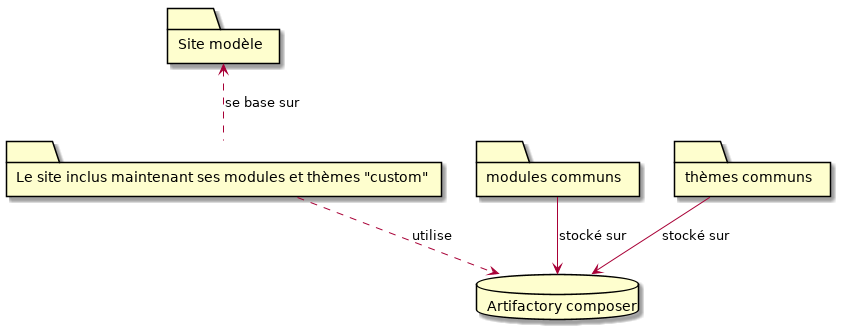
\includegraphics[width=0.50\textwidth]{img/after-drupal.png}
		\end{block}
	\end{overprint}
\end{frame}

\subsection{Versions}
\begin{frame}{Gestion de versions}
	\note[item]{Déploiement auto = version auto. Besoin de savoir ce qui est déployé à un instant T car plusieurs déploiement peuvent être fait par jour.}
	\note[item]{avant: tag git manuel, mais pouvait être oublié sur l'un des trois dépôts. Inconvénient : si erreur de livraison, on ne pense pas forcément à retaguer les trois dépôt après le correctif. Peut être source de problème.}
	\note[item]{Maintenant, modules commun mis à jour à chaque push des développeurs. On peut donc savoir la version d'un site et des modules communs qu'il utilisent à tout instant.}

	\begin{columns}[onlytextwidth]
		\column{.4\textwidth}
		\centering 
\includegraphics[width=1\textwidth]{img/final-version.png}
		\pause
		\column{.5\textwidth}
		\begin{block}{}
			\begin{itemize}
				\item v1.0.0.1
				\item v1.0.0.2
				\item v1.0.1.0
				\item ...
			\end{itemize}
		\end{block}
	\end{columns}
\end{frame}

\subsection{Jenkins}
\begin{frame}{\subsecname}
	\note<1>[item]{Organisé par portail, job identiques, versionnés pour maintenabilité}
	\note<2>[item]{Différents type de job : après push développeur, rapide, chaque nuit, qualité, déploiement, à la demande, possible par toute l'équipe.}
	\note<3>[item]{log par étape afin de savoir les étapes réussies ou non}
	\note<3>[item]{Alerte sur Teams (outil com interne) sur les résultats des builds}
	\begin{overprint}
		\onslide<1>
		\begin{block}{Par projet}
			\centering 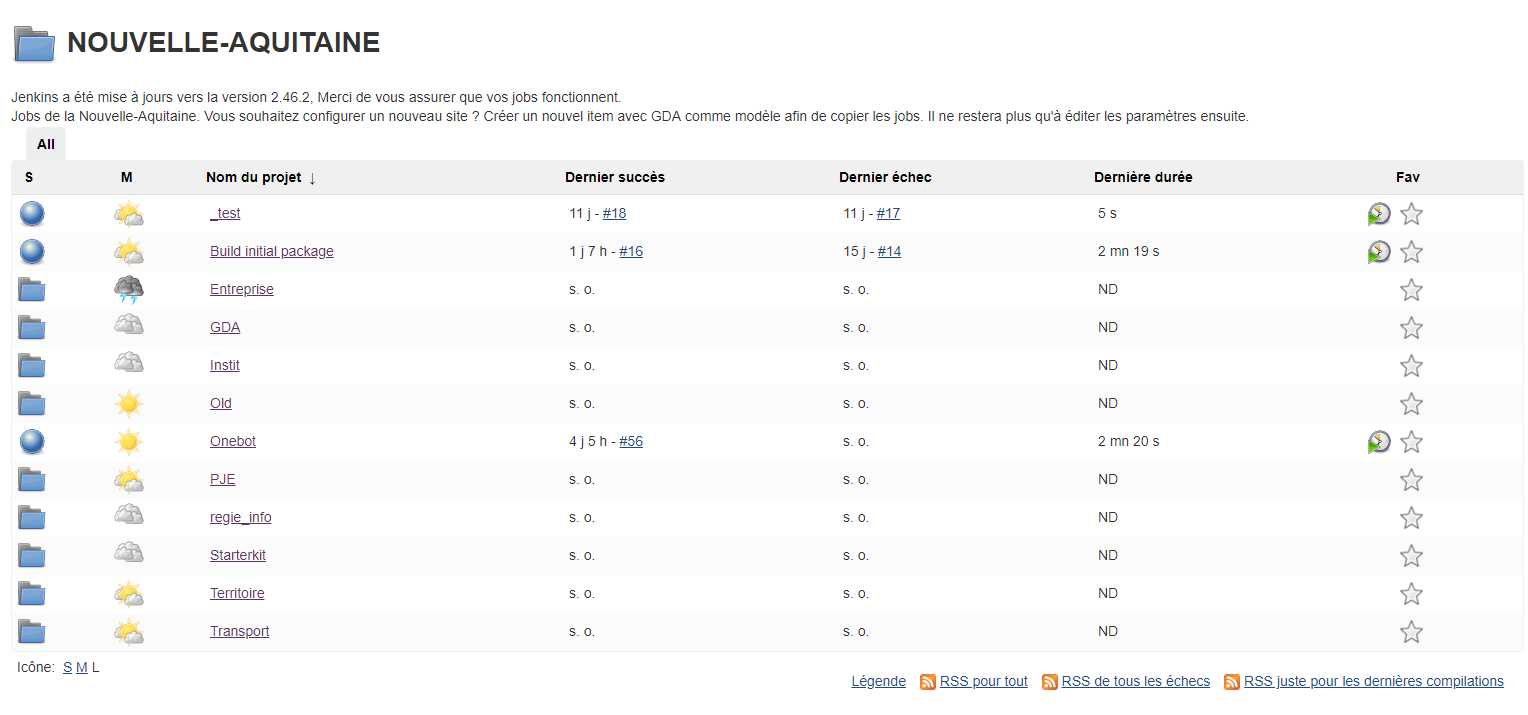
\includegraphics[width=0.8\textwidth]{img/job-naq.png}
		\end{block}
		\onslide<2>
		\begin{block}{Différents besoins}
			\centering 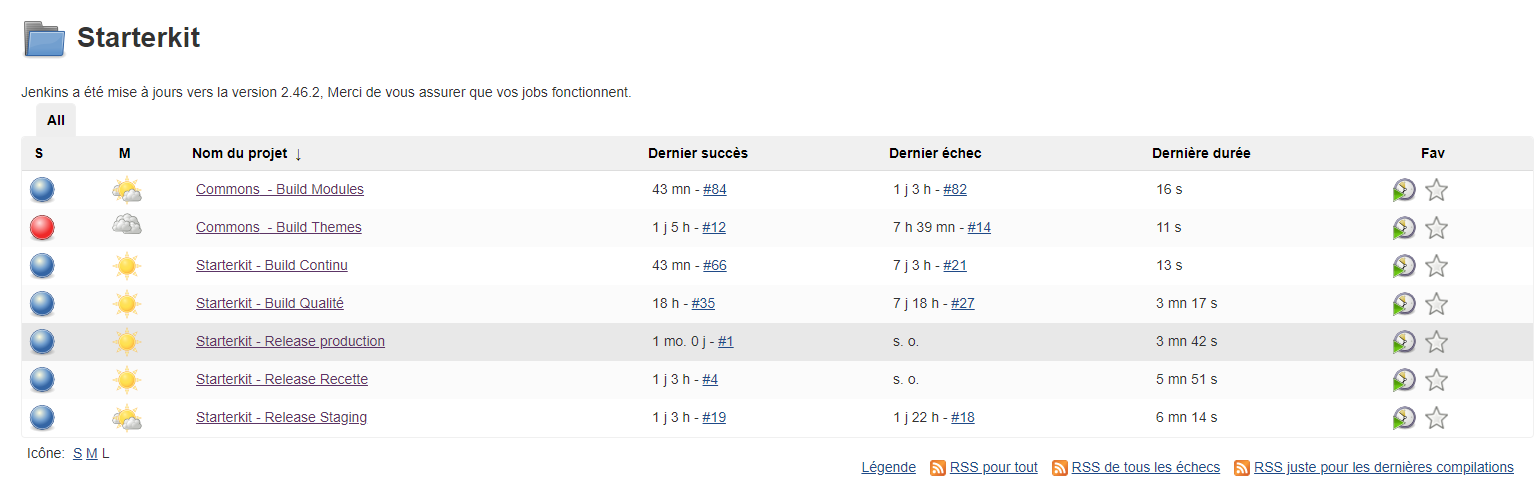
\includegraphics[width=0.8\textwidth]{img/job-starter.png}
		\end{block}
		\onslide<3>
		\begin{block}{Suivi des étapes}
			\centering 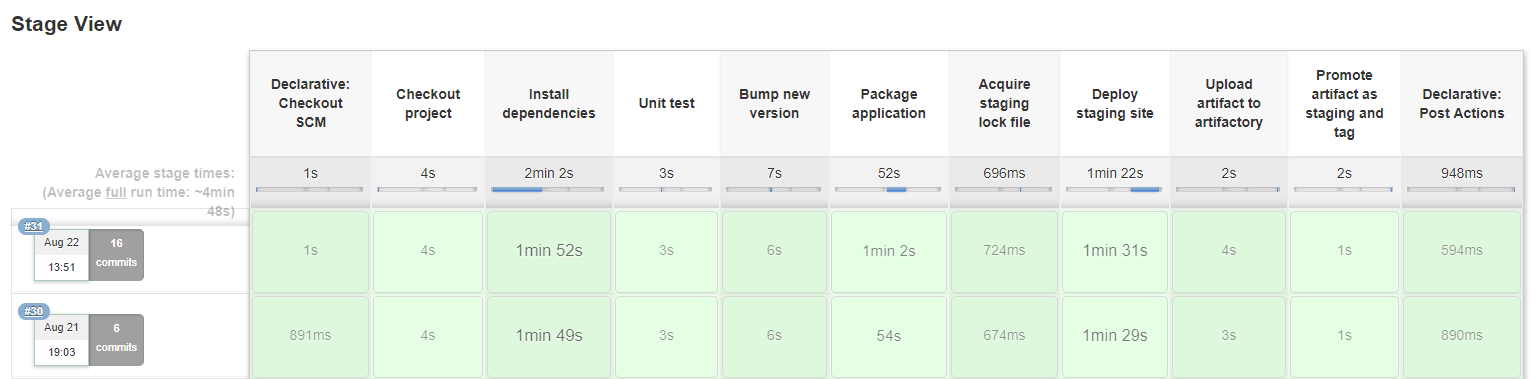
\includegraphics[width=0.8\textwidth]{img/job-regie-staging.png}
		\end{block}
	\end{overprint}
\end{frame}

\subsection{Déploiement}
\begin{frame}{\subsecname}
	\note[item]{Build package de livraison avec ses dépendances, pour éviter erreurs futures \& comportement non souhaités (coupure réseau...) au plus tôt}
	\note[item]{Utilisation d'ansible pour décrire les tâches exécutées. Egalement versionné}	\missingfigure{Récap ansible déploiement}
\end{frame}

\subsection{Sauvegarde}
\begin{frame}{\subsecname}
	\note[item]{Activable par option, permet sauvegarder base données + fichiers. Restauration pas encore automatisée mais prévue.}
\end{frame}

\subsection{Sécurité}
\begin{frame}{Sécurité - Bastion}
	\note[item]{Clé SSH, compte nominatif, permissions restreinte, user de déploiement}
	\note[item]{bastion ssh qui permet de se couper quand pas nécessaire}
	\pause
	\centering 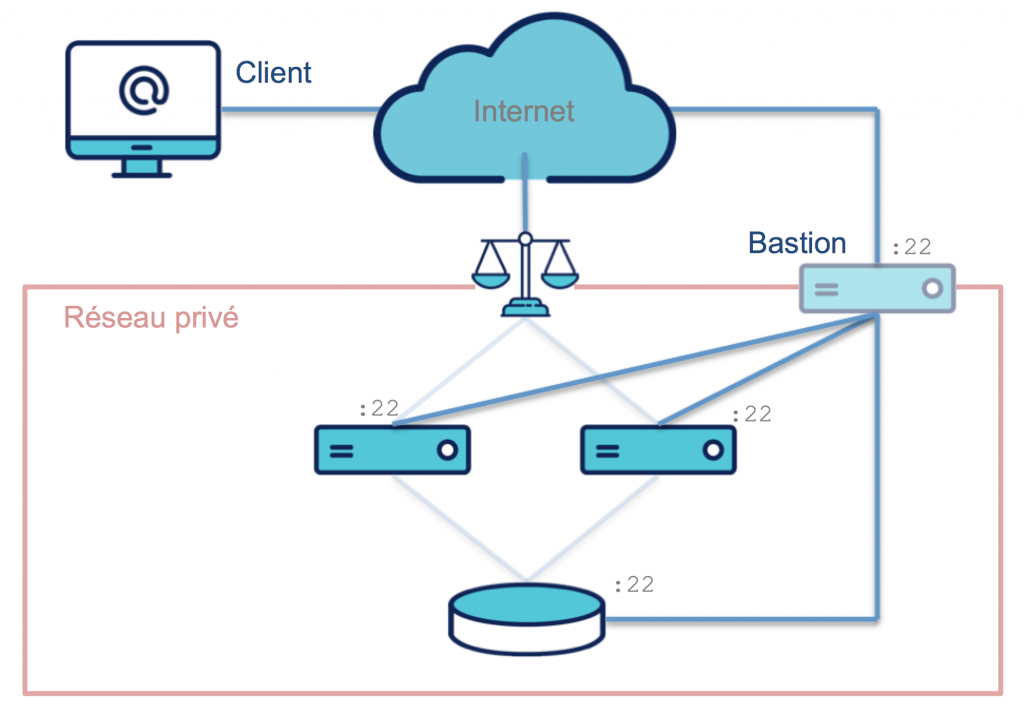
\includegraphics[width=0.60\textwidth]{img/bastion.png}
\end{frame}

	\todo[color=yellow]{Conclusion, 7 pages}

- Pourquoi n'existe pas une solution unique ? => car chaque projet différent 

- Pourquoi complexité des processus de déploiement ? => car complexité application en hausse, et demande utilisateur avec toujours plus de simplicité, et donc complexe à réaliser. Passage d'une "application à la bonne franquette", à un vrai processus éprouvé pour durer

\subsection{Bénéfices}

\todo[color=orange]{Benefices}

\textit{dentifier les leviers d’économie à actionner pour améliorer les processus Qualité.}

\begin{itemize}
	\item KPI à trouver
	\item Confiance dans la livraison
	\item ROI avec rapidité de livraison
	\item Décharge l'équipe
	\subitem Plus de temps pour de la valeur métier
	\item L'automatisation peut permettre de relancer rapidement une activité défaillante (SLA / PRA / PCA)
\end{itemize}

\begin{itemize}
	\item - Erreur développeur
	\item + de Fiabilité
	\item Preuve de qualité
	\item Time To Market réduit
	\item Reproductibilité
\end{itemize}

Comment faire en sorte que ça marche dans la durée ? Des controles / supervisons périodique afin de checker que tout va bien.

Workflow : savoir ce qui est automatisé, comment c'est mis en oeuvre ,documentation des outils, ...
Faire en sorte que l'automatisation ne casse pas et que l'on en tire quelques chose, que l'on soit nouvel arrivant sur le projet, ou développeur déjà présent sur le projet.

Scalabilité : Docker / provisionner de nouveaux serveurs rapidement avec Ansible par exemple.

Déploiement : chaine de déploiement (dev/test/inte/preprod/prod) avec chacune ses spécificités

Exemple :

en dev, on souhaite des logs direct dans la console, en prod on les mets dans un fichier de log.
en dev, on veut le mode debug, en prod on le désactive.

\subsection{Limites}

\todo[color=yellow]{Limites}

Sur-qualité, sur-optimisation, ...

Aucun intérêt si les tests ne sont pas fiable.

Dépend du client, de l'environnement, demande de la flexibilité, délai de mise en place, ROI

Pré-requis à l'automatisation

Attention, auto != vérité \url{https://www.matuzo.at/blog/building-the-most-inaccessible-site-possible-with-a-perfect-lighthouse-score/}

L'automatisation ne peut être utilisée, ou sera risquée, ou plus à même d'amener des régression si de mauvaise pratique sont présentes.

\begin{itemize}
	\item variable codée en dur à la place de variable d'environnement
	\item ...
\end{itemize}

De plus, il faut une certaine organisation.

Cela peut-être perçu comme une perte de temps par certaines personnes (hiérarchie, manager, ...), qui y verrons la une perte d'argent et de temps par exemple. Il faut alors pouvoir montrer que cela est rentable, au travers de \gls{KPI} bien déterminé.

Le fait d'automatiser des processus permet de gagner du temps, et par conséquent de l'argent et de consacrer ses efforts à d'autres taches qui peuvent apporter de la valeur métier.

Le coût horaire libéré, calculer à partir de combien de temps il est rentable.

Par exemple, une tache à 3000€ qu'on automatise et qui ne coute plus que 300€ est rentable en 10 semaines.

Facteur humain : Le temps libéré par l'automatisation des tâches peut permettre de souder les liens d'une équipe et d'améliorer les relations de cette dernière. Cela libère du temps pour du team building par exemple.

Un sujet technique qui rapproche en terme d'humain

Idées de \gls{KPI} en vracs.

Métrique - KPI - temps de déploiement / nombre d'incident / uptime / Nombre de build KO / Nombre de build OK ... permettent de définir l'impact des services mis en place sur le S.I

\begin{itemize}
	\item temps de déploiement
	\item taux de déploiement succès
	\item couverture de code
	\item tests au verts
	\item derniers build KO
\end{itemize}

Parler de l'importance de l'implication du client. 

Ex :  Rédaction de SFD, qui évolue tout les 4 matins, et demande un changement dans l'architecture => automatisation perdante.

Dépôt git du mec qui automatise tout \url{https://github.com/NARKOZ/hacker-scripts}

\subsection{Ce qui n'est pas encore automatisé}

\subsection{Les possiblités d'automatisation dans le futur}

\textit{Parler de ce qui n'est pas encore automatisé, et les différentes pistes d'automatisation possible dans le futur.}



	%----------------%
	
    %----SAMPLES----%
    %\begin{frame}{slide autre}

du blabla

\end{frame}
    %\begin{frame}{slides}

\begin{figure}[htb]
	\centering
	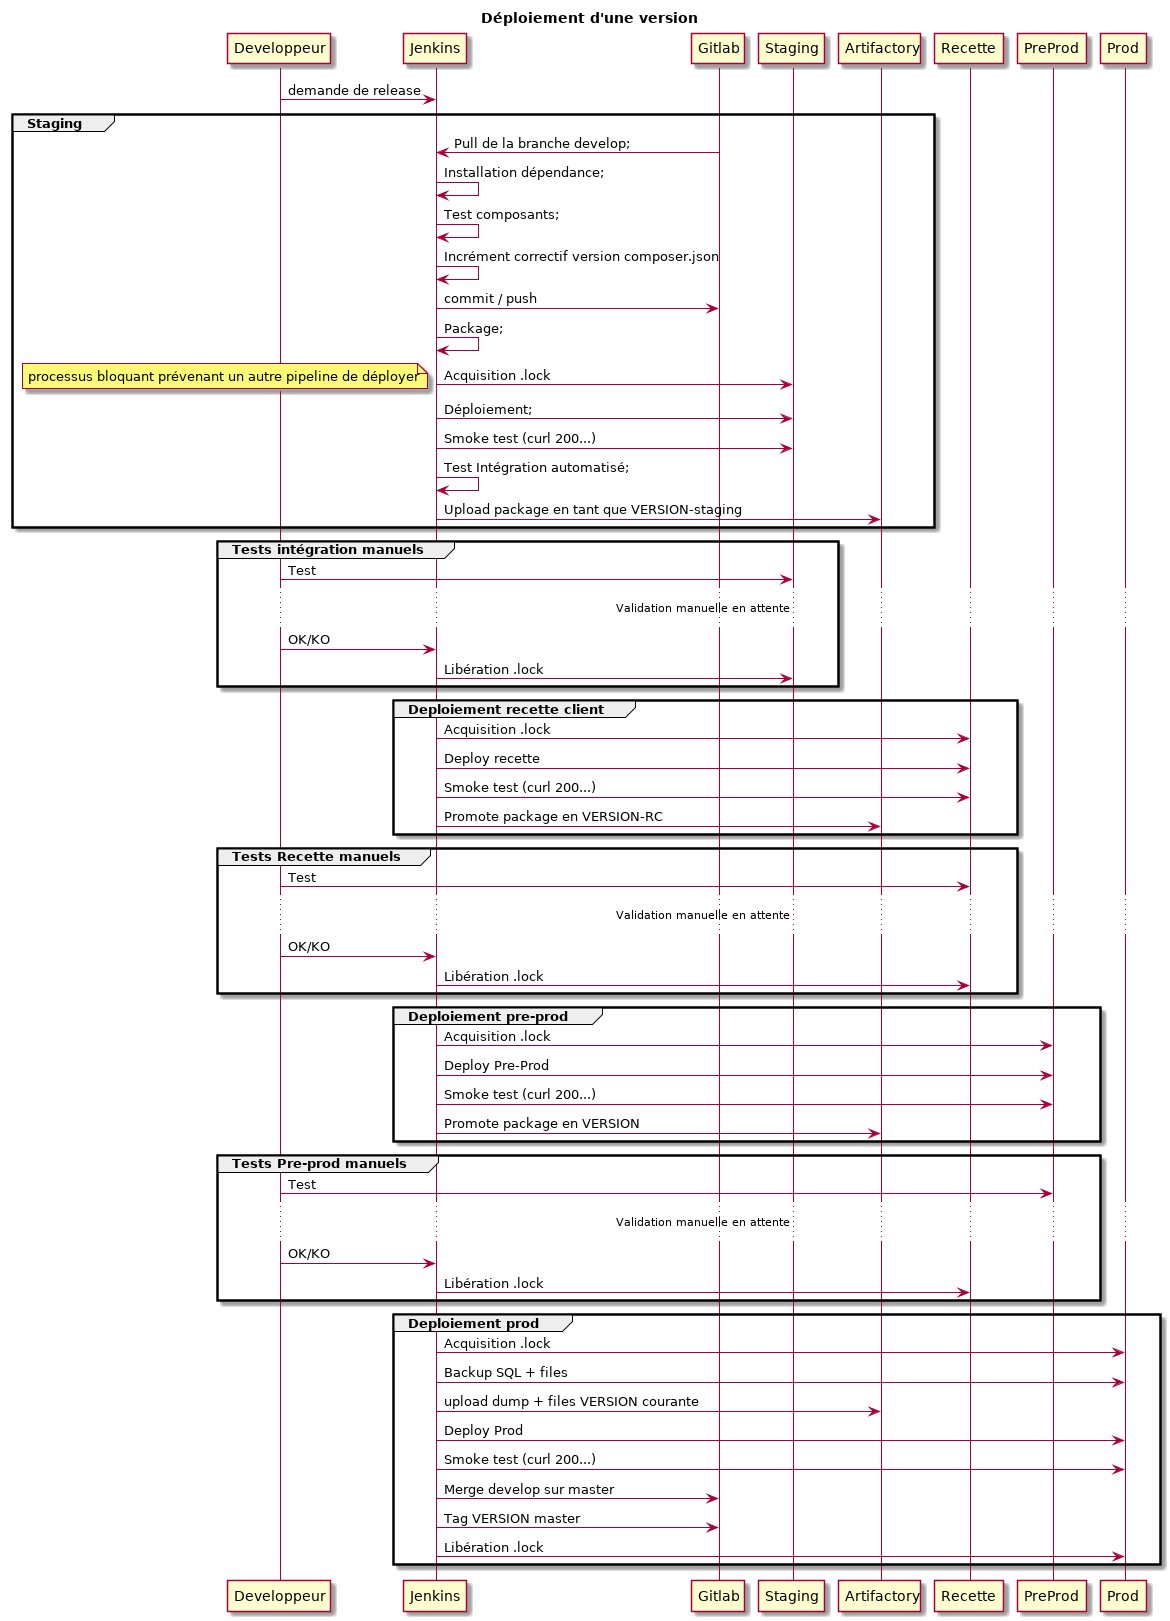
\includegraphics[width=0.3\textwidth]{../img/release.png}
	\caption{Image}
	\label{fig:onepoint}
\end{figure}

\end{frame}
    %\begin{frame}{Slide}

\begin{block}{un bloc}
    des trucs
\end{block}

\begin{block}{autre bloc}
	blablalba
\end{block}

\end{frame}

    %--------------%

\end{document}
